% Unofficial UofT Poster template.
% A fork of the UMich template https://www.overleaf.com/latex/templates/university-of-michigan-umich-poster-template/xpnqzzxwbjzc
% which is fork of the MSU template https://www.overleaf.com/latex/templates/an-unofficial-poster-template-for-michigan-state-university/wnymbgpxnnwd
% which is a fork of https://www.overleaf.com/latex/templates/an-unofficial-poster-template-for-new-york-university/krgqtqmzdqhg
% which is a fork of https://github.com/anishathalye/gemini
% also refer to https://github.com/k4rtik/uchicago-poster

\documentclass[final]{beamer}

% ====================
% Packages
% ====================

\usepackage[T1]{fontenc}
\usepackage[utf8]{luainputenc}
\usepackage{lmodern}
\usepackage[orientation=portrait,size=a0,scale=1.0]{beamerposter}
\usetheme{gemini}
\usecolortheme{uos}
\usepackage{graphicx}
\usepackage{booktabs}
\usepackage{tikz}
\usepackage{pgfplots}
\pgfplotsset{compat=1.14}
\usepackage{anyfontsize}
\usepackage{mathtools}
\usepackage{kotex}
\usepackage{multirow}
\usepackage{multicol}
\usepackage{hhline}


% ====================
% Lengths
% ====================

% If you have N columns, choose \sepwidth and \colwidth such that
% (N+1)*\sepwidth + N*\colwidth = \paperwidth
\newlength{\sepwidth}
\newlength{\colwidth}
\setlength{\sepwidth}{0.025\paperwidth}
\setlength{\colwidth}{0.45\paperwidth}

\newcommand{\separatorcolumn}{\begin{column}{\sepwidth}\end{column}}

\def\cA{{\cal A}}
\def\cB{{\cal B}}
\def\cE{{\cal E}}
\def\cR{{\cal R}}
\def\cH{{\cal H}}
\def\cF{{\cal F}}
\def\cD{{\cal D}}
\def\cL{{\cal L}}
\def\cN{{\cal N}}
\def\cG{{\cal G}}
\def\cK{{\cal K}}
\def\cV{{\cal V}}
\def\cX{{\cal X}}
\def\cY{{\cal Y}}
\def\cP{{\cal P}}
\def\cS{{\cal S}}
\def\cI{{\cal I}}
\def\cC{{\cal C}}
\def\cU{{\cal U}}
\def\smt{{\mbox{\tiny T}}}

\newcommand{\bA}{{\bf A}}
\newcommand{\bD}{{\bf D}}
\newcommand{\bC}{{\bf C}}
\newcommand{\bT}{{\bf T}}
\newcommand{\bt}{{\bf t}}
\newcommand{\bZ}{{\bf Z}}
\newcommand{\bY}{{\bf Y}}
\newcommand{\bz}{{\bf z}}
\newcommand{\bN}{{\bf N}}
\newcommand{\bn}{{\bf n}}
\newcommand{\bfe}{{\bf e}}
\newcommand{\bg}{{\bf g}}
\newcommand{\bff}{{\bf f}}
\newcommand{\bF}{{\bf F}}
\newcommand{\uxj}{x^{(j)}}
\newcommand{\uxk}{x^{(k)}}
\newcommand{\uf}{{\underline f}}
\newcommand{\uH}{{\underline H}}
\newcommand{\bX}{{\bf X}}
\newcommand{\bx}{{\bf x}}
\newcommand{\br}{{\bf r}}
\newcommand{\by}{{\bf y}}
\newcommand{\bW}{{\bf W}}
\newcommand{\bw}{{\bf w}}
\newcommand{\bV}{{\bf V}}
\newcommand{\bv}{{\bf v}}
\newcommand{\bU}{{\bf U}}
\newcommand{\bu}{{\bf u}}
\newcommand{\bI}{{\bf I}}
\newcommand{\bH}{{\bf H}}
\newcommand{\bh}{{\bf h}}
\newcommand{\bfs}{{\bf s}}
\newcommand{\bfa}{{\bf a}}
\newcommand{\hba}{\hat{\bf a}}
\newcommand{\blXn}{{\bf \underline{X_n}}}
\newcommand{\E}{\mbox{{\rm E}}}
\newcommand{\V}{\mbox{{\rm Var}}}
\newcommand{\ri}{\mbox{{\bf \rm ri}}}
\newcommand{\co}{\mbox{{\rm co}}}
\newcommand{\lspan}{\mbox{{\rm lspan}}}
\newcommand{\btheta}{\mbox{\boldmath{$\theta$}}}
\newcommand{\hbtheta}{\mbox{\boldmath{$\hat{\theta}$}}}
\newcommand{\balpha}{\mbox{\boldmath{$\alpha$}}}
\newcommand{\hbalpha}{\mbox{\boldmath{$\hat{\alpha}$}}}
\newcommand{\bepsilon}{\mbox{\boldmath{$\epsilon$}}}
\newcommand{\bbeta}{\mbox{\boldmath{$\beta$}}}
\newcommand{\sbbeta}{\small\mbox{\boldmath{$\beta$}}}

\newcommand{\bgamma}{\mbox{\boldmath{$\gamma$}}}
\newcommand{\bfeta}{\mbox{\boldmath{$\eta$}}}
\newcommand{\bmu}{\mbox{\boldmath{$\mu$}}}
\newcommand{\bSigma}{\mbox{\boldmath{$\Sigma$}}}
\newcommand{\bo}{\boldsymbol{1}}

\newcommand{\bc}{\begin{center}}
\newcommand{\ec}{\end{center}}
\newcommand{\be}{\begin{equation}}
\newcommand{\ee}{\end{equation}}
\newcommand{\ba}{\begin{array}}
\newcommand{\ea}{\end{array}}
\newcommand{\bean}{\begin{eqnarray*}}
\newcommand{\eean}{\end{eqnarray*}}
\newcommand{\bea}{\begin{eqnarray}}
\newcommand{\eea}{\end{eqnarray}}
\newtheorem{proposition}{\bf Proposition}
\newcommand{\ben}{\begin{enumerate}}
\newcommand{\een}{\end{enumerate}}
\newcommand{\bed}{\begin{itemize}}
\newcommand{\eed}{\end{itemize}}
\newcommand{\vs}{\vspace}
\newcommand{\bs}{\boldsymbol}

\newcommand{\mbR}{\mathbb{R}}
\newcommand{\mbE}{\mathbb{E}}
\newcommand{\mbQ}{\mathbb{Q}}
\newcommand{\mbB}{\mathbb{B}}

\usepackage{xcolor, color, soul}
\makeatletter
\let\HL\hl
\renewcommand\hl{%
  \let\set@color\beamerorig@set@color
  \let\reset@color\beamerorig@reset@color
  \HL}
\makeatother

\newtheorem{assumption}{Assumption}

% ====================
% Title
% ====================

\title{RoBaMF : Role-Based Multimodal Fusion model\\
for Online News Classification}

\author{Mose Park \inst{1}} % \and Jong-June Jeon$^*$ \inst{1}}

\institute[shortinst]{\inst{1} Department of Statistical Data Science, University of Seoul, S. Korea}

% ====================
% Footer (optional)
% ====================

\footercontent{
%\href{https://github.com/an-seunghwan/DistVAE}{Code: github.com/an-seunghwan/DistVAE} \hfill
Selective. Lab \hfill
2024 기초연구실 성과발표회 \hfill
\texttt{mose1103@uos.ac.kr}}
% (can be left out to remove footer)

% ====================
% Logo (optional)
% ====================

% use this to include logos on the left and/or right side of the header:
% use this to include logos on the left and/or right side of the header:
% \logoleft{\includegraphics[height=7cm]{logos/UoN_Logo_NottinghamBlue_WhiteText_CMYK.pdf}}
\logoright{
\includegraphics[height=9cm]{logo.png}}

% ====================
% Body
% ====================

\begin{document}



\begin{frame}[t]
\begin{columns}[t]
\separatorcolumn

\begin{column}{\colwidth}

    % \begin{alertblock}{Abastract}
    
    %     \textbf{The transmission of information is not limited to text, but also includes various forms such as images, videos and voices. Thus, the use of multimodal models in data analysis is gaining attention. In this paper, we propose a multimodal model called RoBaMF that reflects both text data and image data from online newspapers in the analysis. The RoBaMF includes a feature-fusion model to reflect the interaction between images and annotations. Additionally, we consider an ensemble methodology that also takes into account single models of text and images. According to our research results, RoBaMF did not improve accuracy compared to article-image composite models, due to some limitations.}
        
    % \end{alertblock}
% ====================
    \begin{alertblock}{Contributions}
    
    \begin{itemize}
        \setlength\itemsep{1em} % Adjusts the space between items
        
        \item \textbf{Introduction of RoBaMF:}
        \begin{itemize}
            \item A new multimodal model for analyzing text and image data from online newspapers.
            \item Enhances understanding of combining different information types for deeper insights.
        \end{itemize}
        
        \item \textbf{Feature-Fusion Approach:}
        \begin{itemize}
            \item Developed within RoBaMF to merge interactions between images and texts.
            \item Aims to capture the full context of news articles more effectively.
        \end{itemize}
        
        \item \textbf{Ensemble Method Exploration:}
        \begin{itemize}
            \item Evaluates and integrates the strengths of individual text and image models.
            \item Leverages the best aspects of both for improved multimodal analysis.
        \end{itemize}
        
        \item \textbf{Insights on Feature Fusion:}
        \begin{itemize}
            \item Emphasizes the importance of \textbf{appropriately feature fusion method}.
            \item Contributes to the enhancement of analysis and interpretation of multimodal data.
        \end{itemize}
    \end{itemize}


    \end{alertblock}
% ====================    


% ====================
  \begin{block}{Introduction}
    % Internet news articles consist of a title, main text, images, and annotations for those images. To categorize these articles, it is reasonable to consider a multimodal model that incorporates both text and image information into the analysis. Moreover, since annotations provide detailed descriptions of the images, there is a strong correlation between images and their accompanying annotations. In this paper, we propose the RoBaMF model, which includes the role of annotations in solving the news article category classification problem. This model incorporates base classifiers using feature-fusion to reflect the interaction between images and their associated annotations. In addition, to reflect the unique information from the article text and images - both of which play significant roles in newspapers - we have incorporated individual base classifiers for each element. The results were produced by applying ensemble methods to these three base classifiers.

    \begin{enumerate}
        \itemsep0.5em % Adjust item separation as needed
        \parskip0.1em % Adjust paragraph separation within an item as needed
        
        \item \textbf{Problem:}
        \begin{itemize}
            \item Internet news articles are complex, consisting of titles, main texts, images, and annotations for those images.
            \item For effective article categorization, integrating text and image information is key.
        \end{itemize}
        
        \item \textbf{Proposed Idea:}
        \begin{itemize}
            \item Recognizing the strong correlation between images and their annotations, we propose the RoBaMF model.
            \item This model uses images and annotations to classify news article categories efficiently.
        \end{itemize}
        
        \item \textbf{Our Methodology:}
        \begin{itemize}
            \item The RoBaMF model fuses features from images and annotations, and adds text and image classifiers.
            \item This method uses ensemble techniques to enhance categorization by utilizing multimodal data.
        \end{itemize}
    \end{enumerate}



  \end{block}

    \begin{figure}[ht]
    \centering
    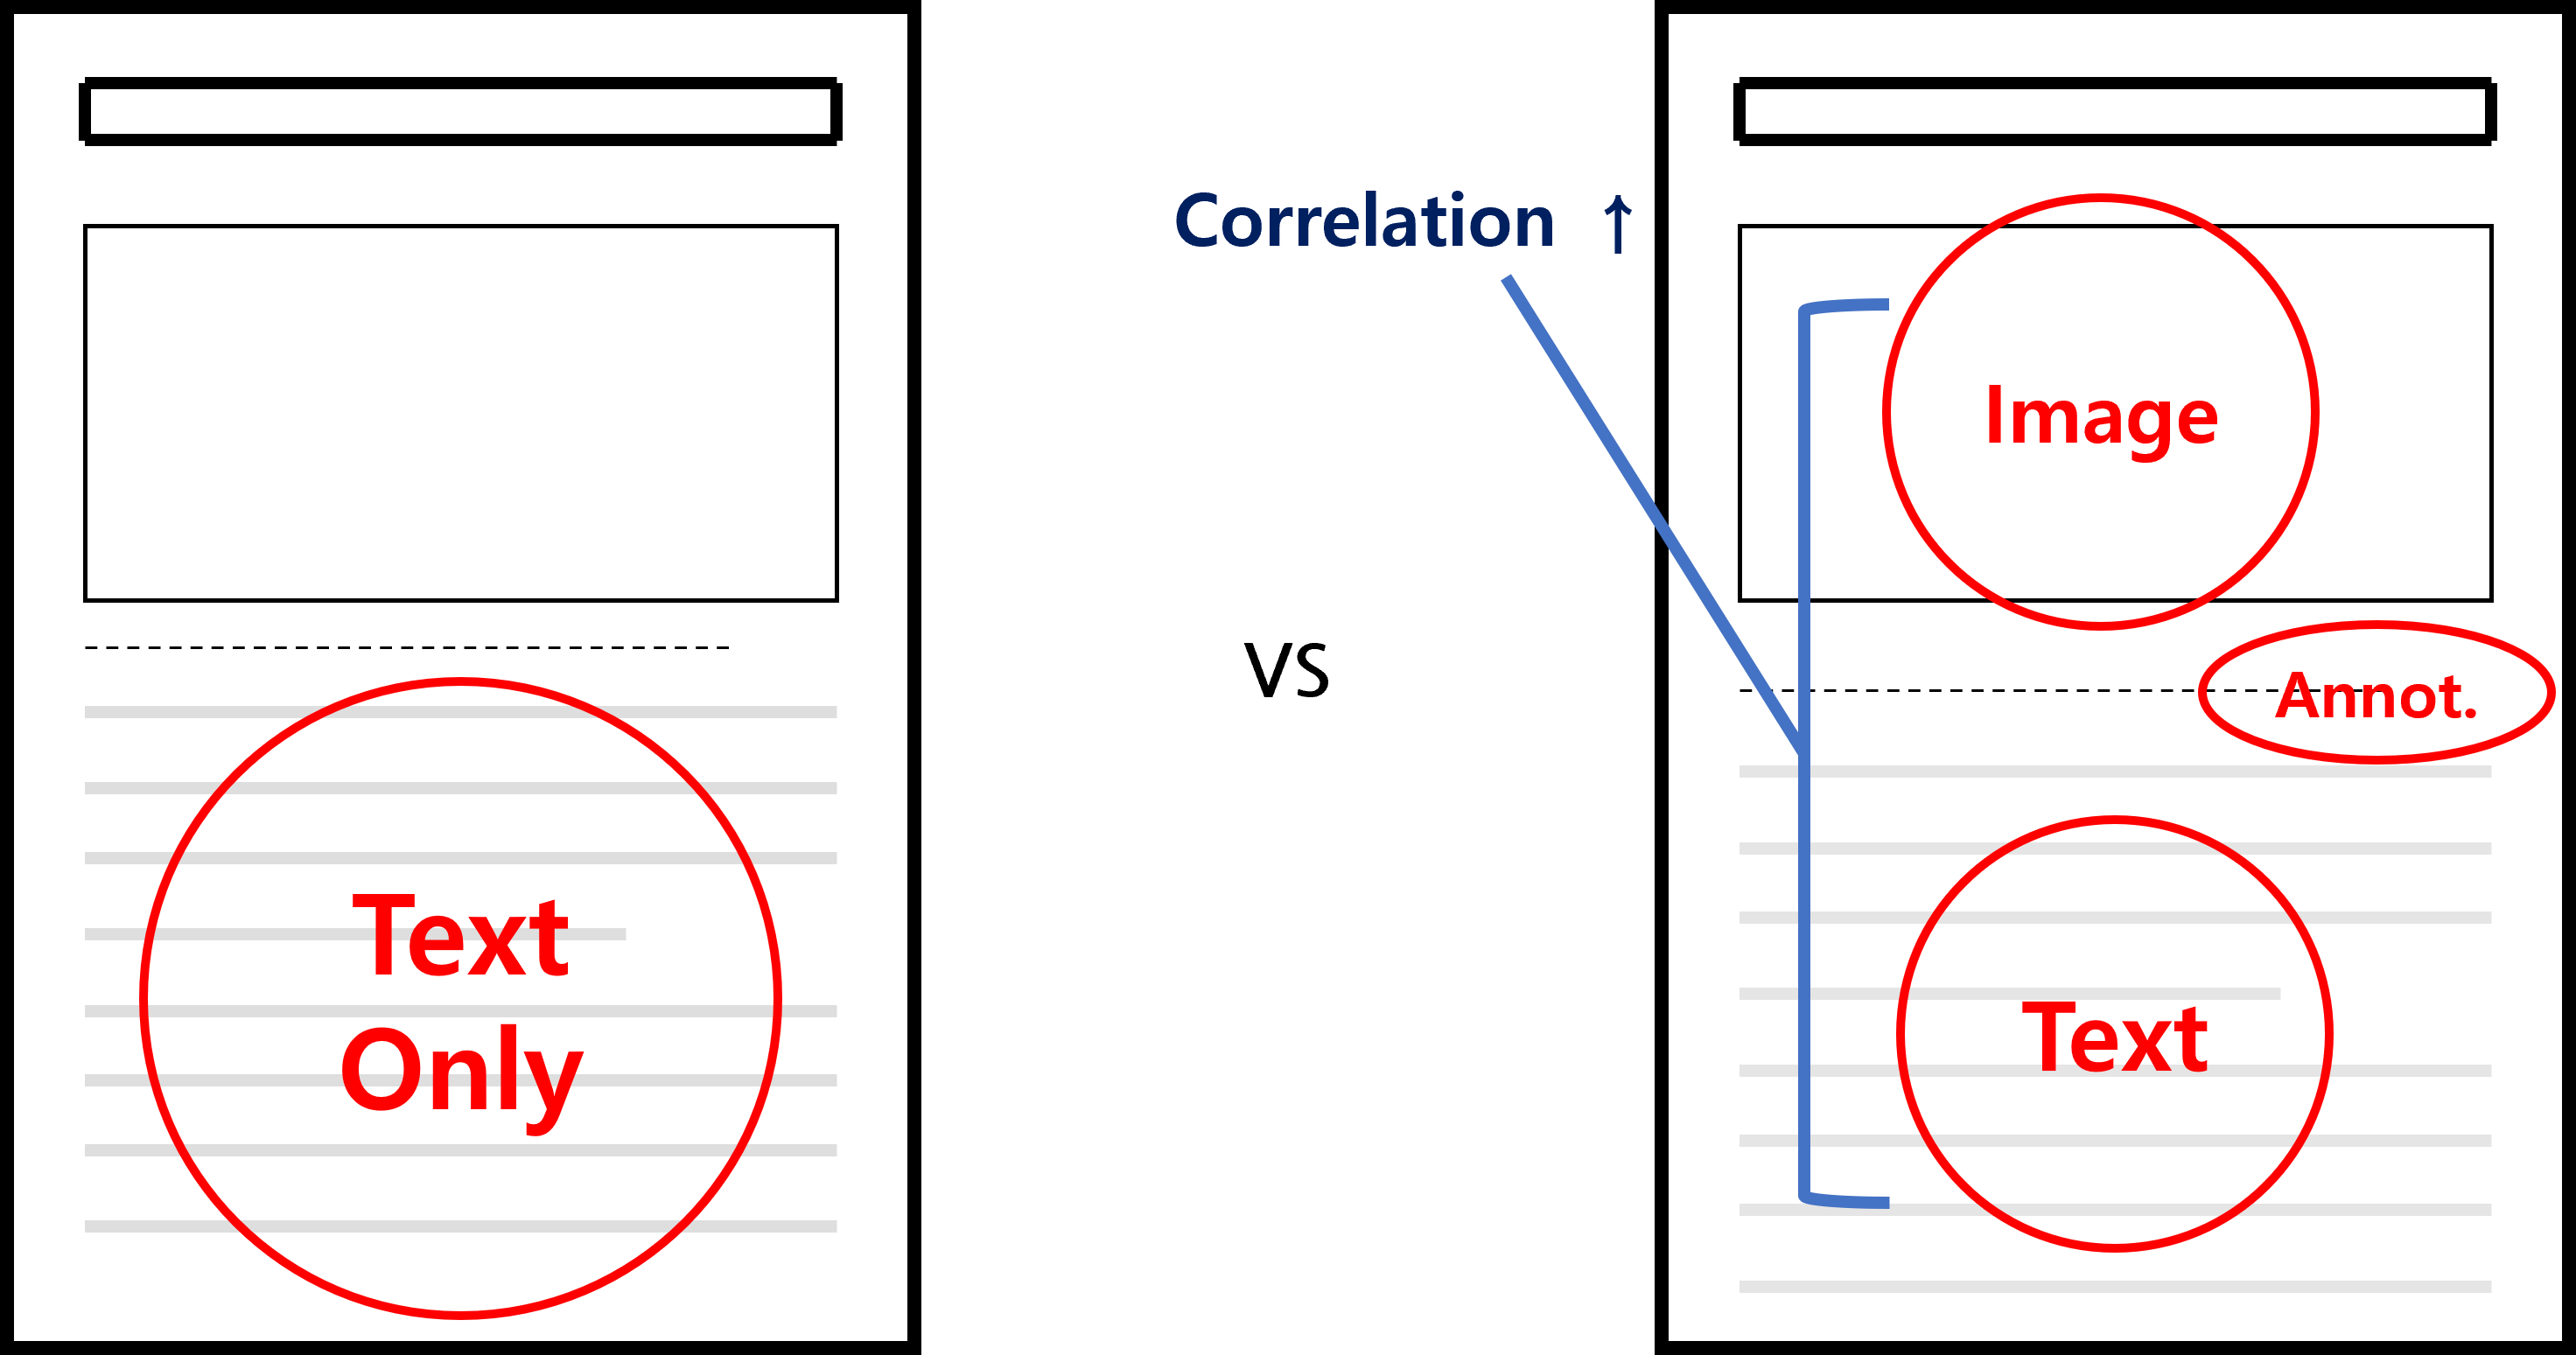
\includegraphics[width=0.5\textwidth]{Figure/fig-target.png}
    \caption{Purpose}
    \label{fig:Purpose}
    \end{figure}

    
% ====================


    \begin{block}{Dataset}
        \setlength{\parindent}{1em}The dataset under consideration contains news title, body, and annotation from \textbf{Naver} captured in the month of \textbf{October 2023}. The goal within this dataset is to \textbf{classify news sections}. There are a total of 6 sections: \textit{Economy, Lifestyle, Politics, Science, Society, and World}. The dataset comprises \textbf{7200} entries, with variables including Title, Image, Body, and Annotation. Here, we will refer to both the Title and Body as the article.
    
        \begin{figure}[ht]
        \centering
        \hspace{2.7cm}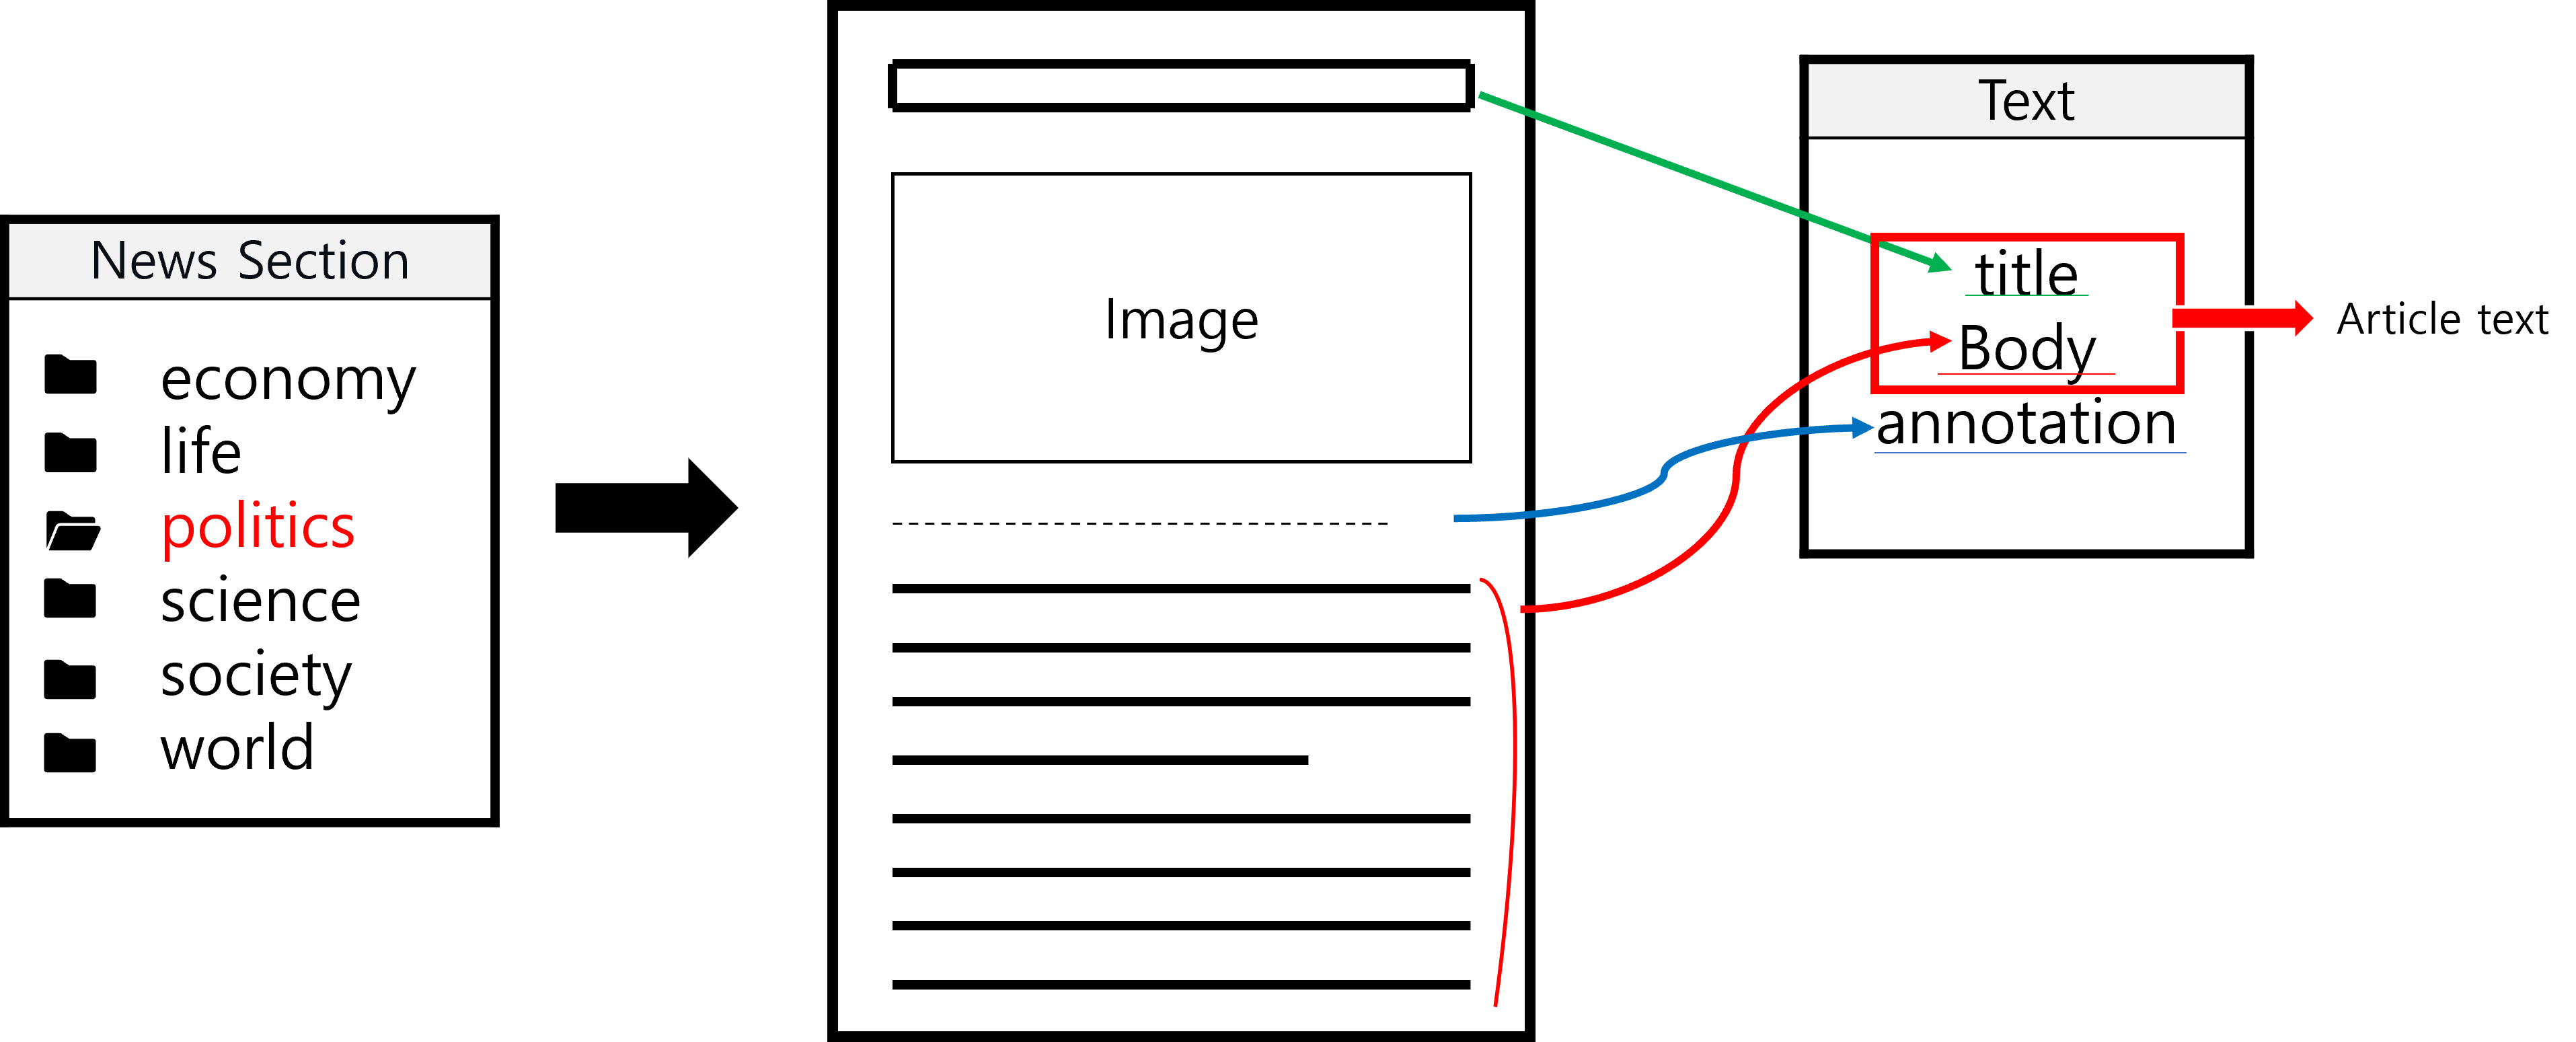
\includegraphics[width=0.75\textwidth]{Figure/fig-dataset.png}
        \caption{Data}
        \label{fig:data}
        \end{figure}
    
    \end{block}


% ====================

    \begin{block}{Feature fusion}
    \hspace{1em}In this research, image features were first extracted using \textbf{MobileNetV2}, and text features were obtained using \textbf{KoBERT}. These features were then input into a feedforward NN model. To do so, two feature vectors were combined by stacking them together into a single vector.
    This feature fusion method, known as concatenation, has several advantages:\\

    \vspace{10pt}

    \textbf{1. Information Preservation}\\
    \begin{itemize}
    \item To concatenate feature vectors, preserving original features.
    \item This method fully preserves features from each domain, minimizing information loss.
    \item It is beneficial for multi-modal data, maintaining the distinct discriminating power of each domain.
    \end{itemize}
    \\
    
    \textbf{2. Flexibility}\\
    \begin{itemize}
    \item Concatenation works regardless of the extraction method, unaffected by changes in the extractor.
    \item This study can replace MV2 with advanced models like ResNet for image feature extraction.
    \end{itemize}
\\


    \begin{figure}[ht]
    \centering
    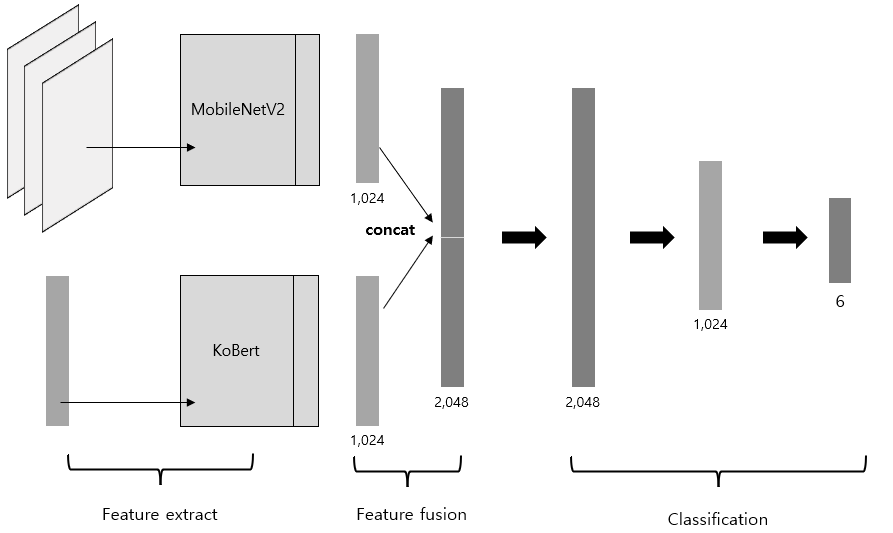
\includegraphics[width=0.67\textwidth]{Figure/feature-fusion-baseline.png}
    \caption{Feature Fusion Framework}
    \label{fig:fusion framework}
    \end{figure}


    \end{block}
% ====================

    

\end{column}

\separatorcolumn

\begin{column}{\colwidth}

  % \begin{block}{Synthetic Data Generation}
  %   \ben
  %       \item Sampling from the prior distribution: $z \sim p(\bz)$.
  %       \item Inverse transform sampling: For $j \in I_C$, $\hat{x}_j = D_j(u_j|z;\theta_j)$, where $u_j \sim U(0, 1)$.
  %       \item Gumbel-Max trick \cite{gumbel1954statistical}: For $j \in I_D$, $\hat{x}_j = \arg\max_{l=1,\cdots,T_j} \{\log \pi_l(z;\theta_j) + G_l\}$, where $G_l \sim Gumbel(0, 1)$, and $l=1,\cdots,T_j$.
  %   \een
  % \end{block}
% ====================
    \begin{alertblock}{RoBaMF : Role-Based Multimodal Fusion Model}
    
    \textbf{\large Stacking Ensemble}
    \begin{itemize}
        \item \textbf{Issue:} The need to accurately predict classifications by leveraging the strengths of multiple base classifiers.
        \item \textbf{Solution:} Utilizing the stacking ensemble methodology, which uses the prediction probabilities from base classifiers as input for a meta-model. XGBoost, a decision tree-based meta-model, is employed to calculate the importance of features.
        \item \textbf{Reason:} This approach allows for an understanding of the impact of image-annotation interaction models on classification, enhancing the multimodal classification model's accuracy and interpretability.
    \end{itemize}
    
    \vspace{5mm} % Adds some space before the next subsection title for better visual separation
    
    \textbf{\large Comparison with Competitor}
    \begin{itemize}
        \item \textbf{Modeling:} The Role-Based Multimodal Fusion Model (RoBaMF) and its competitor are evaluated based on the importance of each baseline in two ensemble models.
        \item \textbf{Reason:} This is to observe the differences between annotation fusion and article fusion.
    \end{itemize}

    \vspace{3em}

    \begin{figure}[ht]
        \centering
        \begin{minipage}[b]{0.45\textwidth}
            \centering
            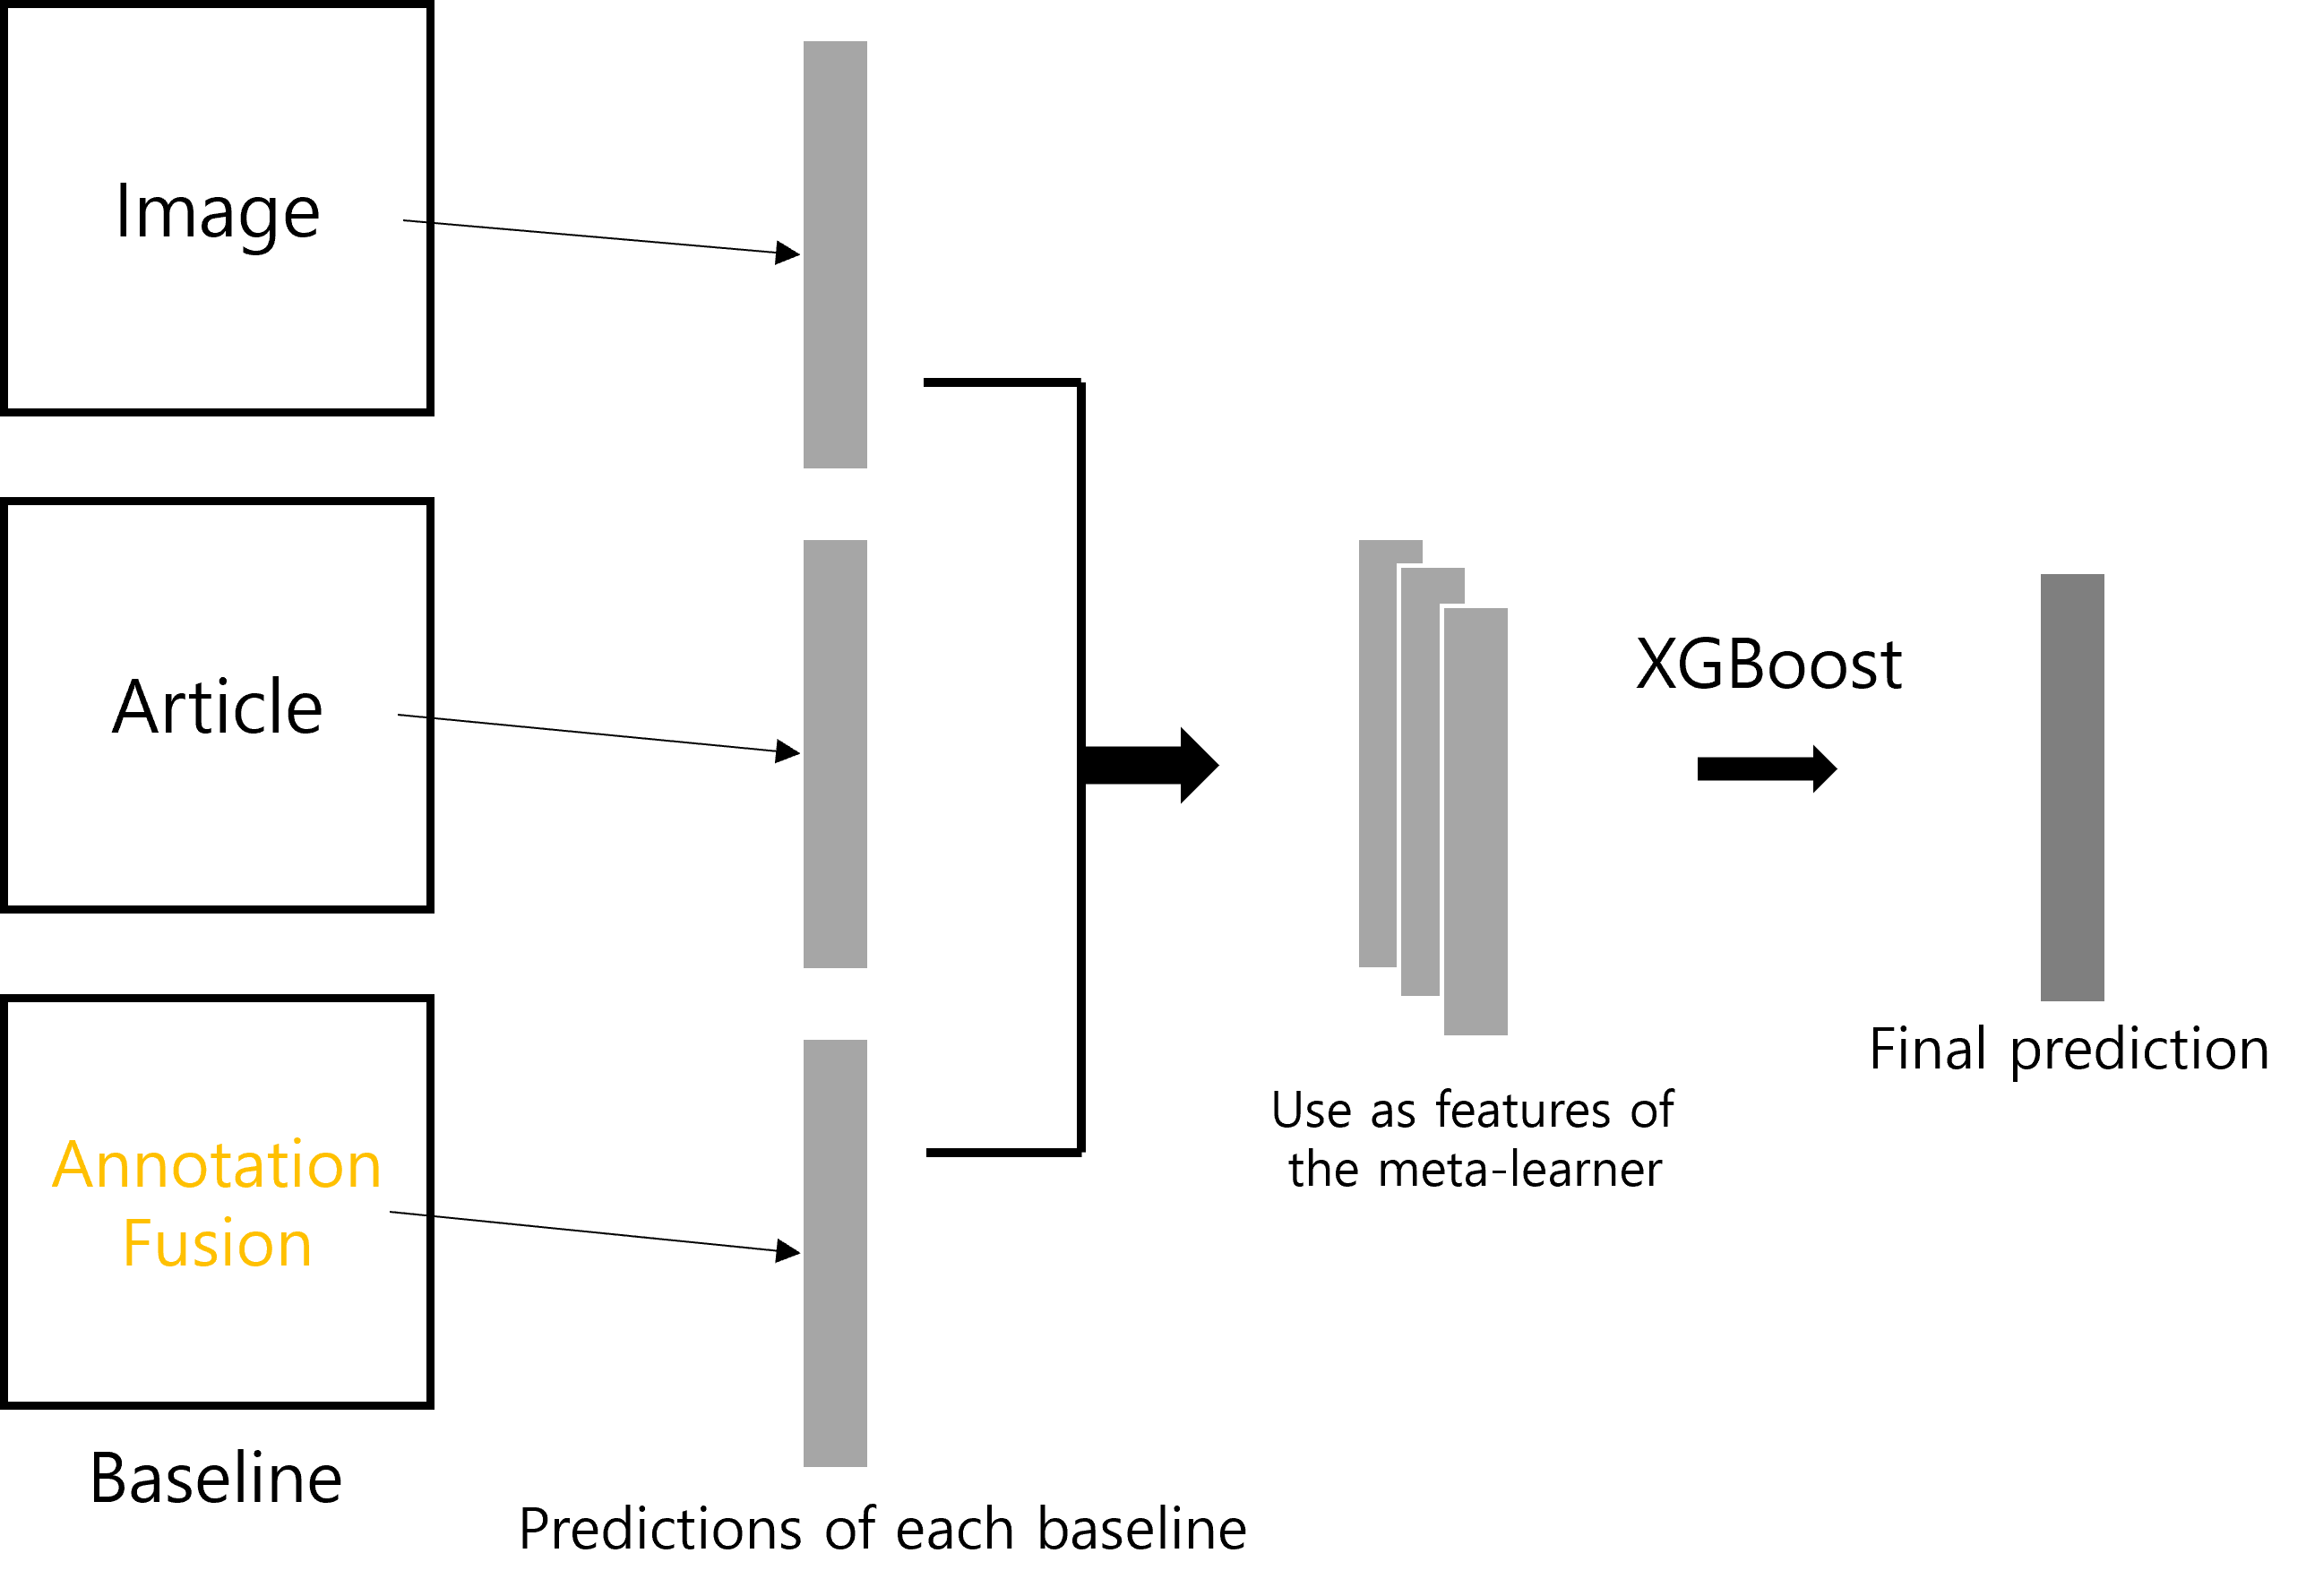
\includegraphics[width=0.8\textwidth]{Figure/fig-model.png} % 첫 번째 이미지
            \caption{RoBaMF}
            \label{fig:model}
        \end{minipage}
        \hfill % 두 minipage 사이의 간격을 조정
        \begin{minipage}[b]{0.45\textwidth}
            \centering
            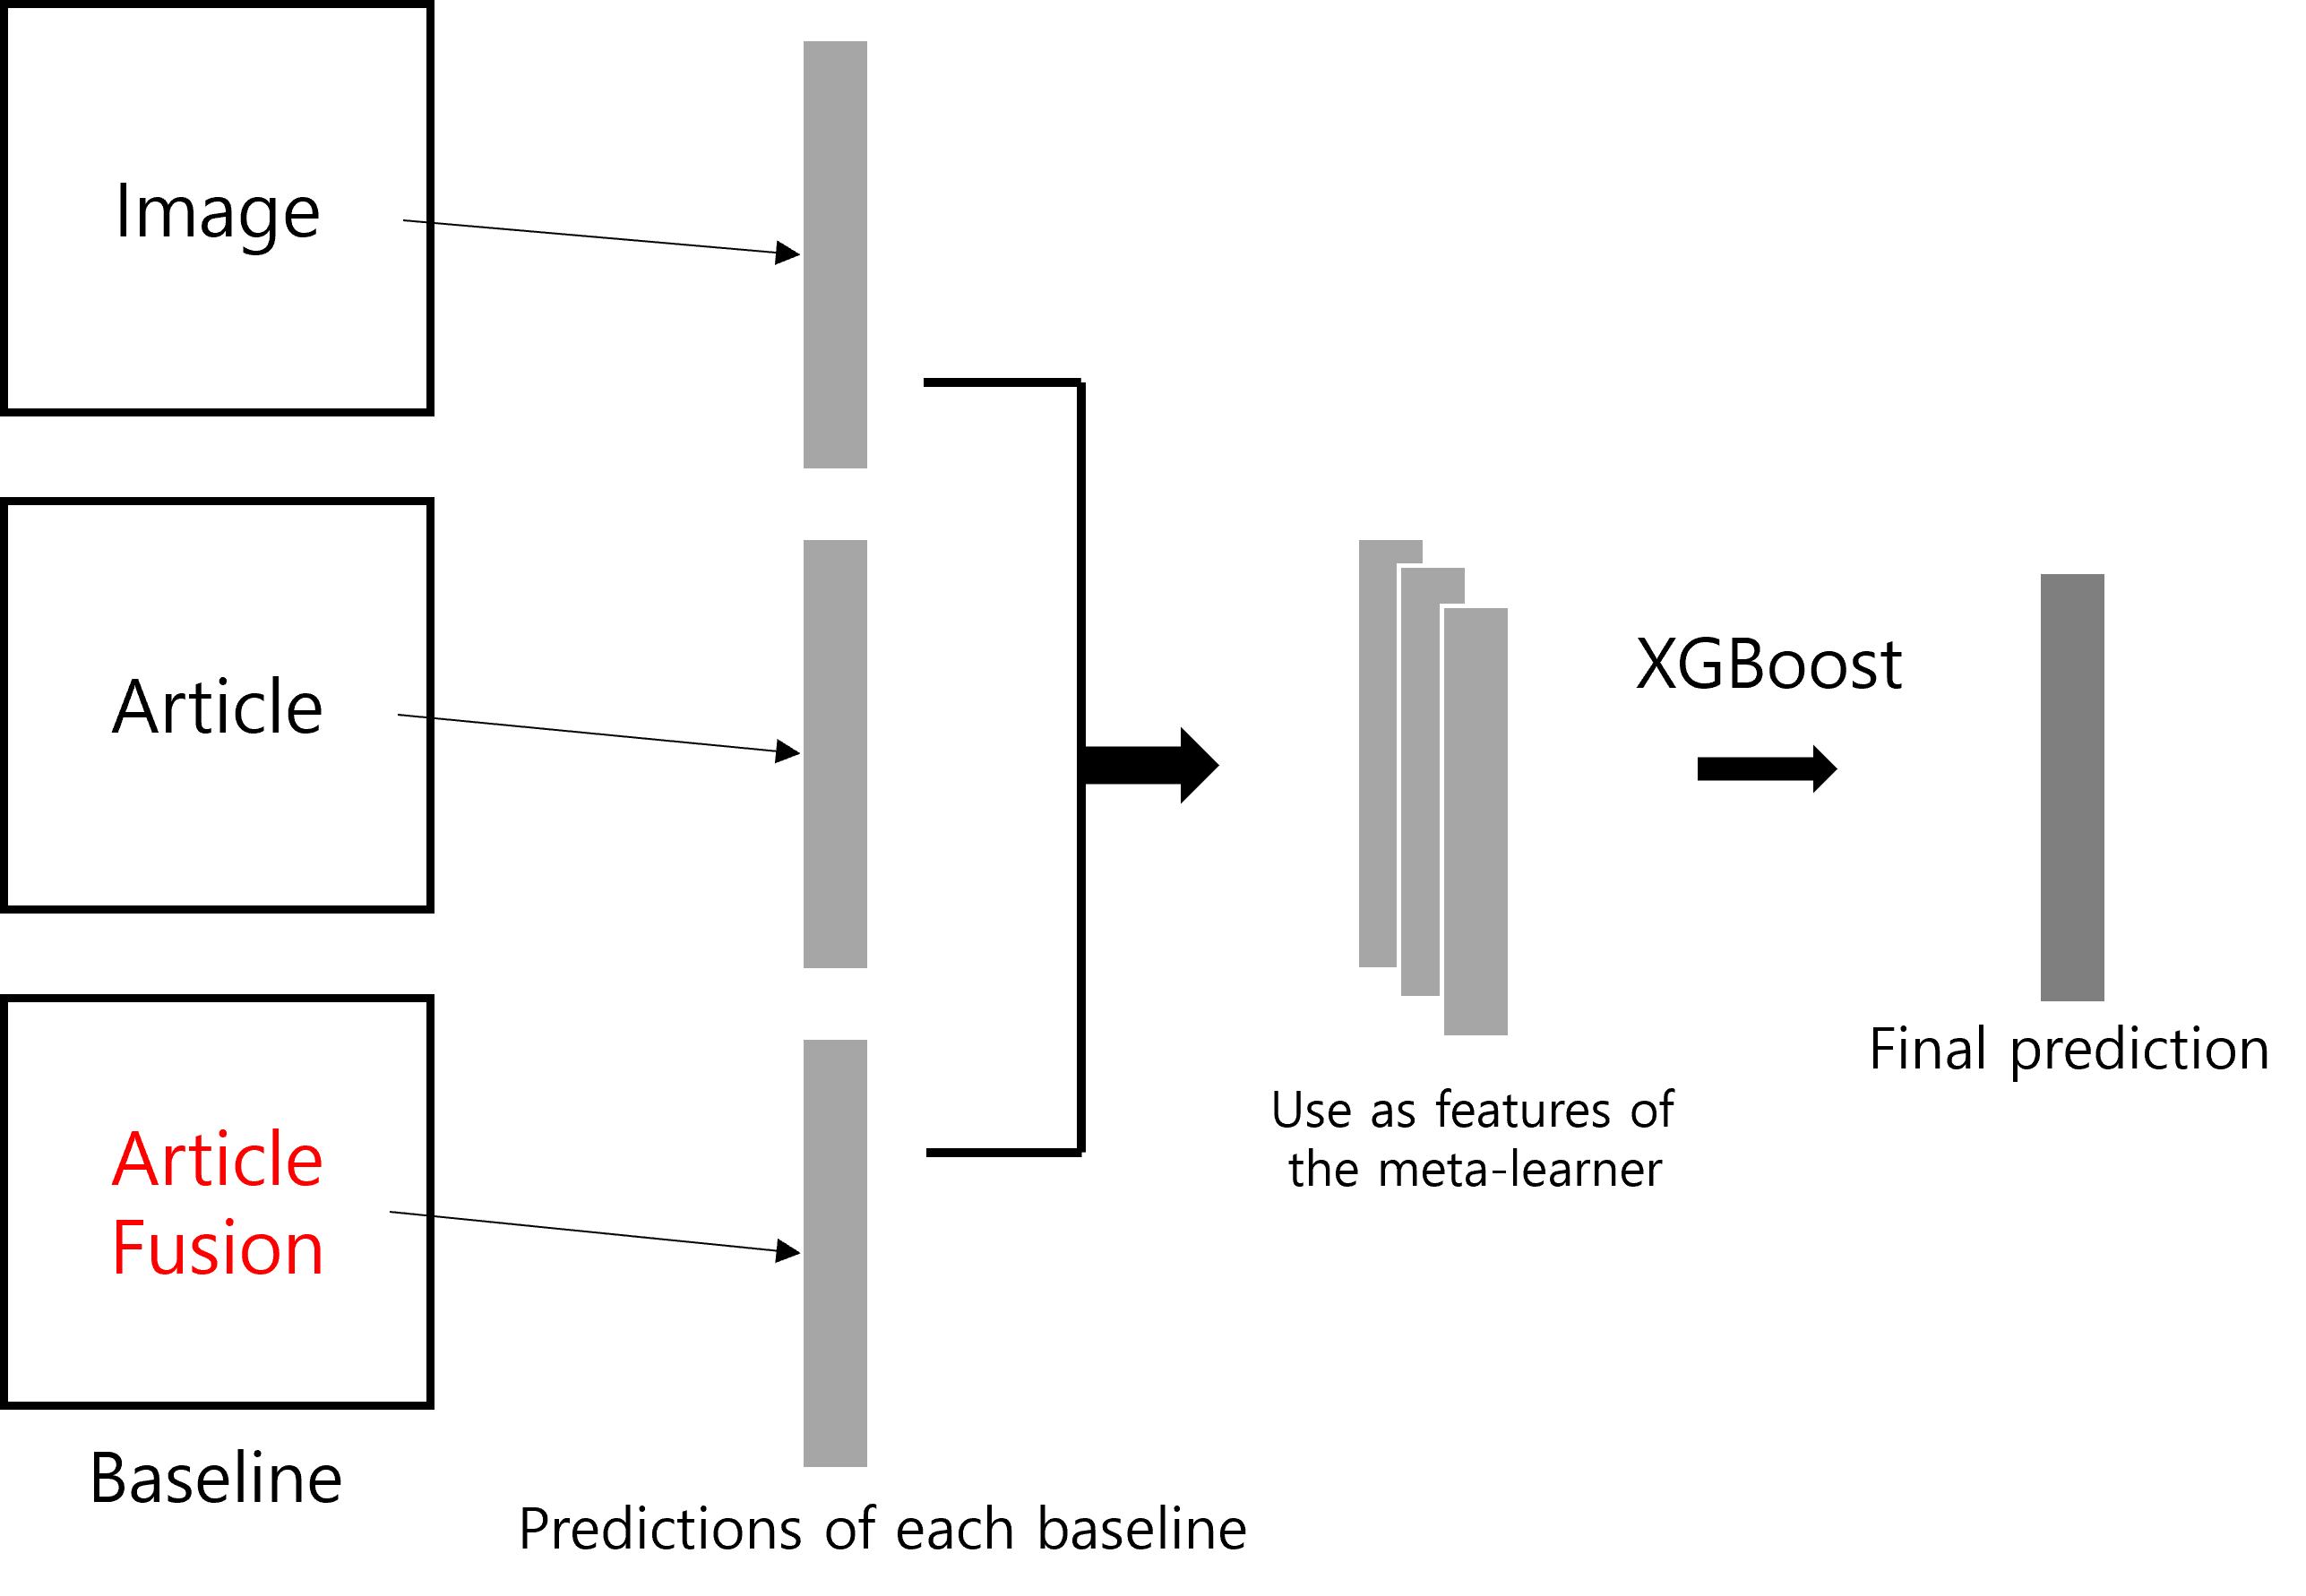
\includegraphics[width=0.8\textwidth]{Figure/fig-competitor.png} % 두 번째 이미지
            \caption{Competitor}
            \label{fig:competitor}
        \end{minipage}
    \end{figure}
        \end{alertblock}

% ====================


  \begin{block}{Experiments}

    \ben
        \item \textbf{Dataset}: 6 real tabular datasets + Image datasets
        \item \textbf{Compared models}: \\
        Baseline (image, article, image+article and image+annot) \\
        Test (baseline, RoBAMF and Competitor)
        \item \textbf{Evaluation Metrics}: Accuracy.
        \item \textbf{Hyper parameter} : learning rate, L2 regularizaiton  and the maximum depth of trees.
    \een



    \heading{Results}

    * \textbf{The K-fold CV accuracies of all baseline classifiers can be seen in Fig.6, and the test data prediction accuracies of all models are presented in Fig.7.} (\texttt{NAVER news} dataset).

    \vspace{5mm}
    
    \begin{figure}[ht]
        \centering
        \begin{minipage}{0.48\textwidth}
            \centering
            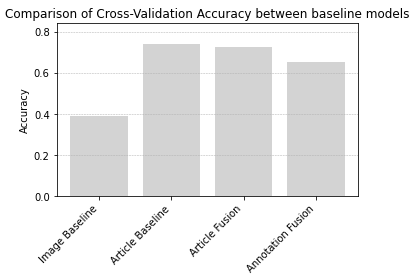
\includegraphics[width=15cm]{Figure/fig-CV-acc.png} % First figure file
            \caption{K-fold CV accuracy of all baseline}
            \label{fig.6}
        \end{minipage}\hfill
        \begin{minipage}{0.48\textwidth}
            \centering
            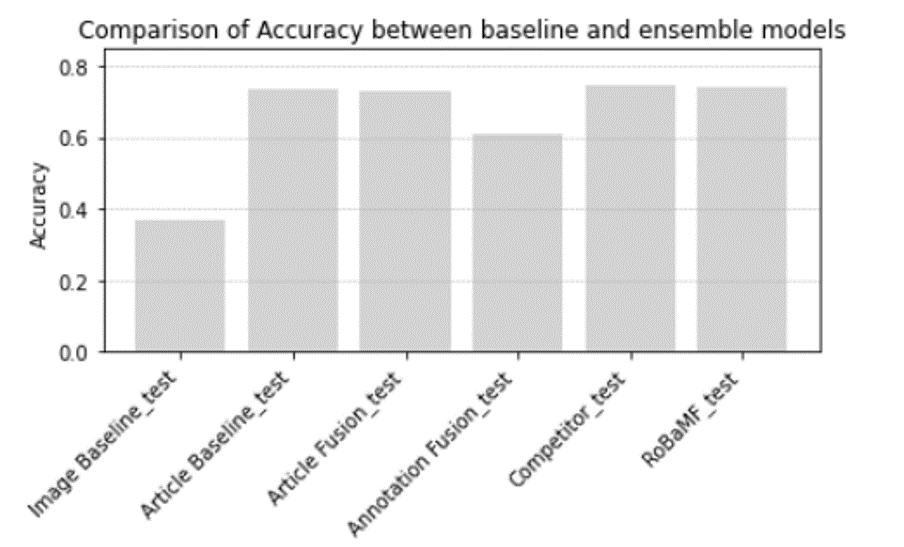
\includegraphics[width=15cm]{Figure/fig-test.png} % Second figure file
            \caption{Test data predictions accuracy}
            \label{fig.7}
        \end{minipage}
    \end{figure}

    \begin{itemize}
        \item \textbf{Left} : Image baseline \textbf{↓}, Article baseline \textbf{↑} and acc(fusion) \textbf{<} acc(article)
        \item \textbf{Right} : Only Article baseline accuracy is superior in test setting.
    \end{itemize}

    %\vspace{20mm}

    \begin{table}[htbp]
        \centering
        \caption{XGBoost: Hyperparameters}
        \label{your-label}
        \begin{tabular}{@{}crrrr@{}}
        \toprule
        \multirow{2}{*}{Scenario} & \multicolumn{4}{c}{Hyperparameter} \\
        \cmidrule(lr){2-5}
        & \multicolumn{1}{c}{n} & \multicolumn{1}{c}{lr} & \multicolumn{1}{c}{lambda} & \multicolumn{1}{c}{max-depth} \\
        \midrule
        1 & 50 & 0.05 & 100 & 4 \\
        2 & 500 & 0.05 & 500 & 5 \\
        3 & 100 & 0.01 & 100 & 3 \\
        4 & 100 & 0.001 & 100 & 4 \\
        5 & 200 & 0.01 & 1000 & 5 \\
        \bottomrule
        \end{tabular}
    \end{table}


    
   \begin{table}[htbp]
    \centering
    \begin{minipage}[t]{0.45\textwidth}
    \centering
    \caption{RoBaMF}
    \label{tab:robamf}
    \begin{tabular}{@{}c|r|ccc@{}}
        \toprule
        \multirow{2.5}{*}{Scenario} & \multicolumn{1}{c|}{ACC} & \multicolumn{3}{c}{Importance} \\
        \cmidrule{2-5}
                 & \multicolumn{1}{c|}{Value} & Image & Article & Fusion \\
        \midrule
        1 & 0.740 & 0.001 & 0.884 & 0.113 \\
        2 & 0.738 & 0.010 & 0.780 & 0.209 \\
        3 & 0.739 & 0 & 0.913 & 0.087 \\
        4 & 0.739 & 0.000 & 0.976 & 0.023 \\
        5 & 0.739 & 0.000 & 0.876 & 0.123 \\
        \bottomrule
    \end{tabular}
    \end{minipage}
    \hfill
    \begin{minipage}[t]{0.45\textwidth}
    \centering
    \caption{Competitor}
    \label{tab:competitor}
    \begin{tabular}{@{}c|r|ccc@{}}
        \toprule
        \multirow{2.5}{*}{Scenario} & \multicolumn{1}{c|}{ACC} & \multicolumn{3}{c}{Importance} \\
        \cmidrule{2-5}
                 & \multicolumn{1}{c|}{Value} & Image & Article & Fusion \\
        \midrule
        1 & 0.745 & 0.003 & 0.699 & 0.297 \\
        2 & 0.745 & 0.011 & 0.565 & 0.423 \\
        3 & 0.750 & 0.001 & 0.751 & 0.247 \\
        4 & 0.748 & 0.000 & 0.819 & 0.179 \\
        5 & 0.747 & 0.000 & 0.751 & 0.248 \\
        \bottomrule
    \end{tabular}
    \end{minipage}
\end{table}

\begin{itemize}
    \item The RoBaMF model has an average \textbf{importance} of \textbf{11\%}, while the competitor has \textbf{29\%}.
    \item The low performance is due to the fusion model obtaining a lower information gain.
    
\end{itemize}





  \end{block}

    \begin{alertblock}{Conclusion}
    % \textbf{Discussion:}
    % \begin{itemize}
    %     \item Image baseline has low performance due to ambiguous image data.
    %     \vspace{5pt} % 항목 간 간격 추가
    %     \item Fusion baseline exhibits lower accuracy rates than Article baseline. This is attributed to:
    %     \begin{itemize}
    %         \item Loss of discriminating power caused by feature concatenation.
    %         \item Failure in choosing the optimal optimizer and hyperparameters.
    %     \end{itemize}
    %     \vspace{5pt} % 항목 간 간격 추가
    %     \item Annotation fusion baseline underperforms due to insufficient information in annotation texts.
    %     \vspace{5pt} % 항목 간 간격 추가
    %     \item The RoBaMF model, despite using more data than the Competitor model, performed worse. This is due to:
    %     \begin{itemize}
    %         \item The differing discriminating power between the two fusion baselines.
    %     \end{itemize}
    % \end{itemize}

    
    % % \bc
    % % $\Downarrow$
    % % \ec
    \textbf{Further research:}
    \ben
        \item Explore methods for fusing features in news data without compromising discriminating power of modalities.
        \item Investigate if news-specific pre-training (e.g., KLUE-BERT) can address the limitations in annotation text information.
    \een
    
    \end{alertblock}

  % \begin{block}{References}

  %   % \nocite{*}
  %   \footnotesize{\bibliographystyle{plain}\bibliography{poster}}

  % \end{block}

\end{column}

\separatorcolumn
\end{columns}
\end{frame}

\end{document}
